\section{Designing Bayesian Networks for Prediction}\label{bayesian_network}
This section will describe the Bayesian networks we made to predict the enemy spawn position, enemy build order, and enemy threat level. The next subsection describes the network created for predicting the enemy spawn position.

\subsection{Prediction of Enemy Spawn Position}			 
			
The purpose of this Bayesian network is to find our opponent's spawning position. Some factors taken into account are our spawn position, enemy scout positions, and time to help us predict this. We wanted to make this network usable on a variety of maps. Below is a visual representation of how each node is connected in the network.
%Why do we represent time as almost none, early, middle, and late?
%actual time for these times - refrace.

\begin{figure}[H]
	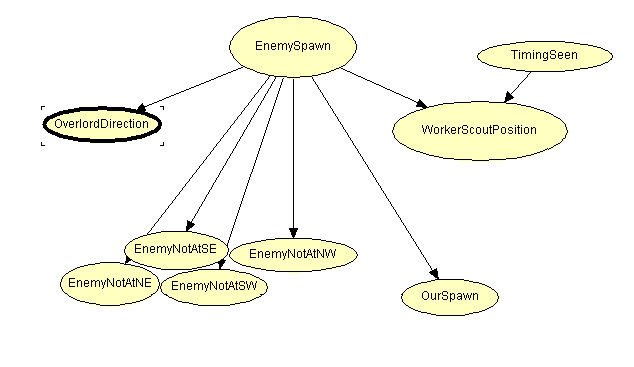
\includegraphics{Figures/BayesianPictures/SpawnPrediction.png}
	\caption{A graph of the nodes in the Spawn Prediction Bayesian network}
	\label{fig:predicting}
\end{figure}

\subsubsection*{EnemySpawn}
The correct state in this node is the value we are trying to discover. Ultimately, all of the evidence we collect, will be used to find this state. Most of the other nodes have direct links from this node. Once we know the state of this, we are satisfied and do not need to use the network to infer more information because we do not care about predicting any of the other states.

\subsubsection*{OurSpawn}
This node is a child of EnemySpawn. We can use the values in this node to determine where the enemy does not spawn. We simply say that the enemy cannot spawn where we spawn at. At the beginning of a match we know where we spawn and can instantly put evidence on the OurSpawn node. This instantly reduces the change for our opponent to be at any other spawning location to 33\%.

\subsubsection*{EnemyNotAt(NE,SE,SW,NW)}
These nodes are used to keep track of positions we know our opponent did not spawn. Since a node can only be in one state at a time, we made four nodes that can influence the probabilities in enemy spawn. Ways we would generally get these values could be our own scouts arriving at a position and not finding our opponent.

\subsubsection*{WorkerScoutPosition} When we observe an enemy worker at a certain position on the map, we can influence our belief on our opponents spawn position. This is because the opponent's scout will take a certain amount of time to get to a certain position on the map. TimingSeen is a parent of this node. We use the information from this node to help our prediction. Just seeing an enemy at a certain position isn't enough. We need the time we see the enemy scout to help us form our beliefs. Whenever we obtain evidence on WorkerScoutPosition we will also always gather information on TimingSeen.

\subsubsection*{TimingSeen} This node is used to help us use the information from WorkerScoutPosition. It has the values: Almost None, Early, Middle, and Late. These values are the times we may see the opponent's scout. Since the values for timing depend on both map size and map layout, we purposely make the values broad.


\subsubsection*{OverlordDirection} Since overlords are so slow, a player will be able to use the direction the overlord is coming from to predict the spawn location. By the time an overlord would have visited two bases we probably would have already known where the enemy's base is. This node only helps when fighting against Zerg players. EnemySpawn is a parent of OverlordDirection. Once we know the direction the overlord is coming from we gain a lot of information on the enemy's spawn position.

\subsection{Build Order Prediction}
	This subsection describes the Bayesian networks that were created for predicting which build order the enemy is doing. 
	The networks have some similarities between them. There are three different networks, one each for every race that the bot can encounter: 
	Terran versus Terran, Terran versus Protoss and Terran vs Zerg.  \\
	
	They all have a node called BuildChosen, which is the node containing the beliefs for what the enemy's build order is. 
	The other nodes are buildings (Except an upgrade node in the Terran vs Protoss network) all with the states Seen and NotSeen. Seen is only used when presenting evidence because the bot will never be able to prove that the enemy building does not exist. 
	These states determine if we have scouted the building. 
	The order in which the buildings appear in the network is modelled with arrows going from the nodes representing the prerequisite buildings needed to the node. 
	As buildings are scouted evidence is put on the state Seen. The nodes and the probabilities for the most probable build order is then increased.

\subsubsection{Terran versus Terran}
	This network will try to predict the following build orders: Proxy Rush, 2 Factory Vulture Pressure, 1 Factory Expand, 1 Starport Wraith and Stim Rush. 
	The numbers in the node names are how many of the given unit the enemy has, e.g. Barracks2 means the second barracks the bot scouts. 
	
\begin{figure}[H]
	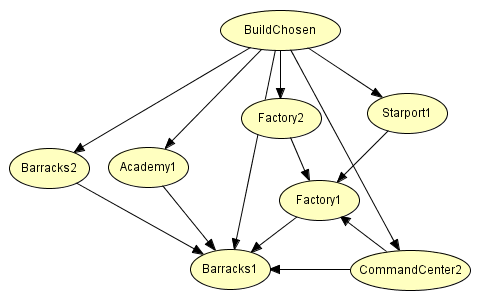
\includegraphics{Figures/BayesianPictures/tvt.png}
	\caption{Terran versus Terran prediction network}
	\label{fig:tvtnetwork}
\end{figure}			
\subsubsection{Terran versus Protoss}
	This network is larger than the other two prediction networks. Instead of only having a node for BuildChosen it has a node for the opening 
	used. The reason for this is that the Protoss are a very versatile race, and the different openings effect when the build order hits and what kind of build 
	the player is most likely to use. After the opening is determined all the nodes affecting the openings are not updated any more. The build orders 
	the network can predict are : 2 Base Carrier, 2 Base Reaver and 2 Base Arbiter. The openings the bot can predict are: One Gate Tech, Two Gate Range, 
	Nexus First and Two Gate Zealot Rush.

\begin{figure}[H]
	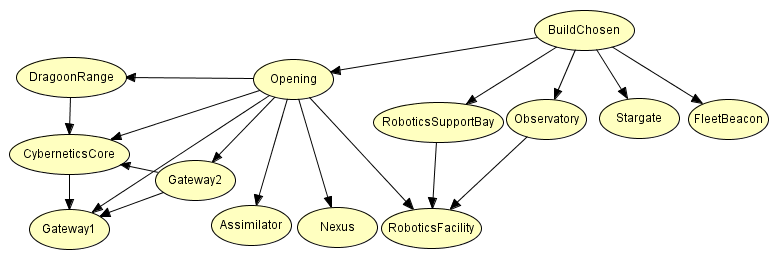
\includegraphics[scale=0.8]{Figures/BayesianPictures/tvp.png}
	\caption{Terran versus Protoss prediction network}
	\label{fig:tvpnetwork}
\end{figure}	

\subsubsection{Terran vs Zerg}
	This network will try to predict the following build orders: 2 Hatch Muta, 3 Hatch Muta, 3 Hatch Lurker and Early Pool Rush. Early Pool Rush is a 4pool or 5pool. The nodes have names similar to the Terran network where a node's name ends on the number of that type is scouted. 
	E.g Hatchery3 means that the bot have scouted 3 hatcheries.

\begin{figure}[H]
	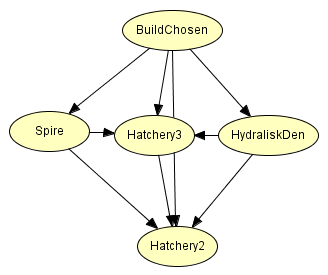
\includegraphics[scale=1]{Figures/BayesianPictures/tvz.png}
	\caption{Terran versus Zerg prediction network}
	\label{fig:tvznetwork}
\end{figure}	
		
			
\subsection{ThreatLevel Prediction}
	This prediction is closely related to the prediction of the enemy build order. A build order has a certain time where it is effective 
	or where it hits. To determine what the current threat level is two nodes have to be added to each of the build order prediction networks, 
	ThreatLevel and Time. ThreatLevel has the states Low, Medium, and High. To make the network simple it only has three states for time: 0-5 minutes, 
	6-8 minutes and 9-11 minutes. By presenting evidence like before and putting evidence on the time node, the current threatlevel can be read.
\begin{figure}[H]
	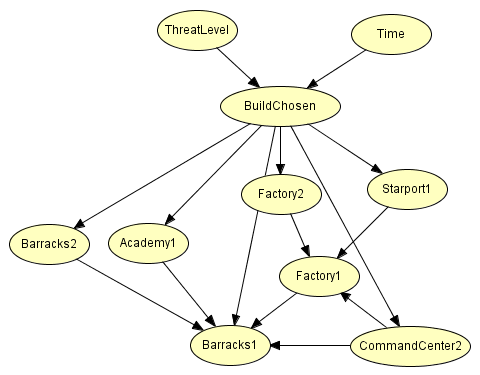
\includegraphics[scale=1]{Figures/BayesianPictures/threatlevel.png}
	\caption{ThreatLevel for the Terran vs Terran matchup}
	\label{fig:threatlevel}
\end{figure}	










 
